% Created 2017-04-27 Thu 02:12
% Intended LaTeX compiler: xelatex
\documentclass[a4paper, notitlepage]{report}
\usepackage{graphicx}
\usepackage{grffile}
\usepackage{longtable}
\usepackage{wrapfig}
\usepackage{rotating}
\usepackage[normalem]{ulem}
\usepackage{amsmath}
\usepackage{textcomp}
\usepackage{amssymb}
\usepackage{capt-of}
\usepackage{hyperref}
% set the margins here, if they need to be modified
\usepackage[a4paper, left=1.3in, right=1.0in]{geometry}

% The linespacing you want
\linespread{1.4}

% Lets you pick fonts. Only works if you compile with xelatex or luatex
\usepackage[no-math]{fontspec}

% For block quotes
\usepackage{attrib}

% Additional mathsy symbols
\usepackage{amsmath}
\usepackage{amssymb}

% Used to make the captions on figures sans serif
\usepackage{caption}

% For including images
\usepackage{graphicx}

% For fancy code listings
\usepackage{listings}

% For tables that span multiple pages elegantly
\usepackage{longtable}

% For APA-style citations

% For maintaining a list of abbreviations
\usepackage{nomencl}

% For drawing diagrams
\usepackage{tikz}

% These closely match the SCSS word template fonts
% Won't work unless you compile with xelatex or luatex
\setmainfont[Mapping=tex-text]{Times New Roman}
\setsansfont{Helvetica}
\setmonofont{Courier New}

\pagestyle{headings}

\hypersetup{
    colorlinks,
    citecolor=black,
    filecolor=black,
    linkcolor=black,
    urlcolor=black
}

\bibliographystyle{acm}

% Settings for how you want your code listings to look
\lstset{
basicstyle=\ttfamily\scriptsize,
keywordstyle=\ttfamily,
numberstyle=\rmfamily\tiny,
numbers=left,
commentstyle=\sffamily,
breaklines=true,
frame=single,
stringstyle=\ttfamily,
identifierstyle=\bfseries,
lineskip=1mm
}

% Change these as appropriate, and they'll be filled in automatically on the
% cover page. You can also use them throughout the document, so as not to have
% to type them again all the time.
\newcommand \authorname{Brian McNestry}
\newcommand \authoremail{mcnestrb@tcd.ie}
\newcommand \supervisorname{Dr. Donal O'Mahony}
\newcommand \degreetitle{B.A. (Mod.) Integrated Computer Science}
\newcommand \projecttitle{Electricity Trading Between Smart Nano-Grids: \newline Matching Supply and Demand in the Face of Unpredictable Supply}

% All the commands are defined in this file
\newcommand \inserttitlepage{\thispagestyle{empty}
\begin{center}
{\sffamily
{\Large University of Dublin}

\vspace{10pt}


\includegraphics[scale=0.5]{tcd/trinitycollege.pdf}

\vspace{10pt}

{\Huge TRINITY COLLEGE}

\vspace{80pt}

\textbf{ \Large \emph \projecttitle}

\vspace{30pt}

\authorname

\degreetitle

Final Year Project May 2017

Supervisor: \supervisorname

\vspace{100pt}

\large{School of Computer Science and Statistics
\\$ $\\
O'Reilly Institute, Trinity College, Dublin 2, Ireland}
\linespread{1}
}
\end{center}

}
\newcommand \insertabstract{\begin{abstract}
\thispagestyle{plain}
As fossil fuels across the world are steadily depleted, the majority of the
world's energy production will shift towards renewable sources. However,
renewable energy sources do not always guarantee the same reliability in rates
of production. Therefore new strategies must be developed to match supply and
demand in the face of unpredictable supply. The growing popularity and
proliferation of smart grid technology is one proposed method of solving this
problem.

In this paper, a network implementation of a game theoretic approach to this
problem is implemented in a smart nanogrid to prove whether or not such an
approach is first feasible in a network, and secondly whether or not it would
provide a better approach to the problem. A number of optimisation techniques,
such as convex optimisation and hyperplane projection optimisation, are also
employed to find a better solution. 
\end{abstract}
}
\newcommand \declaration{\chapter*{Declaration}

I hereby declare that this project is entirely my own work and that it has not
been submitted as an exercise for a degree at this or any other university.
$ $\\
$ $\\
\signedanddate
}
\newcommand \acknowledgements{\chapter*{Acknowledgements}

Acknowledge the various people here
}
\newcommand \permissiontolend{\chapter*{Permission to lend}

I agree that the Library and other agents of the College may lend or copy
this report upon request.

$ $\\
$ $\\
\signedanddate
}

\newcommand{\argmax}[1]{\underset{#1}{\operatorname{arg}\,\operatorname{max}}\;}

\usepackage{datetime}

\def\fullhrulefill{\leavevmode\leaders\hrule height 1pt\hfill\kern 0pt}

\newcommand{\signedanddate} {
  \par\noindent\makebox[2.5in]{\fullhrulefill}
  \par\noindent\makebox[2.5in][l]{\authorname, May 5 2017}
}

\newcommand \needcite[1]{\underline{#1}}

\newcommand \abbrev[2]{#1\nomenclature{#1}{#2}}


% For changing the names of the List of Listings, etc.
\renewcommand*{\lstlistlistingname}{List of Listings}
\renewcommand*{\contentsname}{Table of Contents}
\renewcommand*{\nomname}{Abbreviations}

% Make the captions sans serif
\renewcommand{\captionfont}{\sffamily}

\addbibresource{bibliography.bib}
\author{Brian McNestry}
\date{\today}
\title{}
\hypersetup{
 pdfauthor={Brian McNestry},
 pdftitle={},
 pdfkeywords={},
 pdfsubject={},
 pdfcreator={Emacs 24.5.1 (Org mode 9.0.5)}, 
 pdflang={English}}
\begin{document}

\inserttitlepage

\pagenumbering{roman}

\declaration

\permissiontolend

\insertabstract

\acknowledgements

\tableofcontents

\newpage

\pagenumbering{arabic}

\part{Introduction}
\label{sec:org69ccaed}
\part{Background}
\label{sec:org89ac0a9}
\chapter{Decentralised Grid}
\label{sec:orga84df6f}
At present in Ireland and in many other countries, the national electric grid
infrastructure is controlled by a central body, namely the ESB. While there are
several electricity providers in Ireland, such as Bord Gáis Energy, SSE
Airtricity and Energy Ireland, each of them use the same distribution network as
one another. Essentially the power is provided from each of the different
providers and then routed into the same centralised hub belonging to the ESB.
From there, each consumer (a household) receives the energy that they pay for
accordingly at a fixed rate through that same infrastructure belonging to the
ESB. This is much the same system as any other country, where there is a
centralised grid. 

This system has been in place for decades and lends itself very well to the
situation where large companies can provide a steady supply of energy by way of
electricity plants that use both renewable and non-renewable energy sources.
Non-renewable energy sources, also known as fossil fuels, include resources such
as coal, gas and oil. While these are finite resources, at present they can be
burned at a steady rate in order to meet the demands of customers. Electricity
from renewable sources can also be produced at a fairly steady rate by placing
large farms in areas that are particularly well suited to the type of renewable
energy being produced. For example, large wind farms are set up in windy
regions far removed from residential or urban areas and solar panels can be
placed in regions that typically enjoy clearer skies than other areas.

However in the future, perhaps the very near future, with the ongoing depletion
of non-renewable resources, more and more people will turn to deploying solar
panels and local wind farms in their locale, regardless of whether or not they
are living in a particularly sunny or windy area. At the moment there are a few
houses out there that use a solar panel to heat their water or other smaller
tasks but soon more and more people will become more and more dependent on what
they can produce either within their own home, or in a more collective sense in
their own neighbourhood to power their houses.

The issue that then arises in these areas that aren't as sunny or windy is that
supply of electricity is no longer steady. The current system could not be
maintained as the energy produced on a local level would be small enough that it
would not be worth it to pass this energy upstream to the central grid. The
energy would instead be used at a local level to try to cover the demand for
electricity of the house or business with which that particular device is
associated.

The model of infrastructure that would then be required is that of a
decentralised grid. This model would need a massive infrastructure overhaul in
order to implement so it would not exist in the world until it is needed and
accepted by the major companies who would then go about implementing it. In this
case necessity would be the mother of invention, at least on a practical level.
The rough idea of a distributed grid is described in figure 1.1. Throughout the
rest of this report distributed grid and decentralised grid are used
interchangeably. 

\begin{figure}[htbp]
\centering
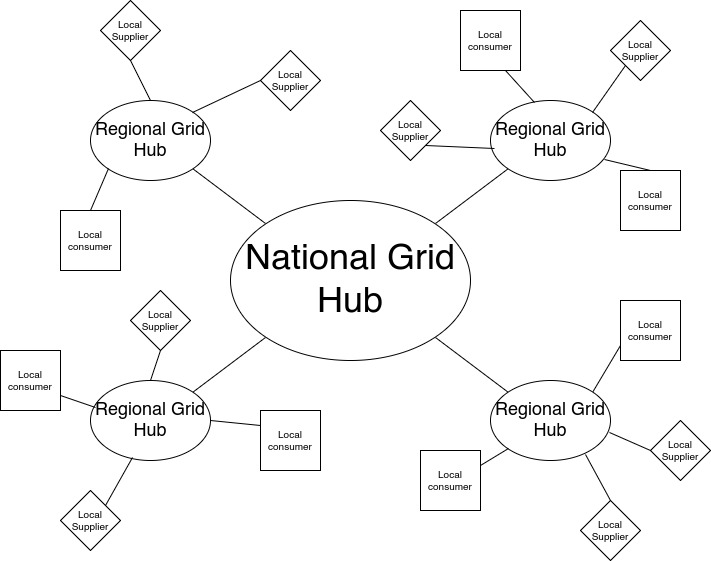
\includegraphics[width=.9\linewidth]{./img/DecentralisedGrid.jpg}
\caption{\label{fig:org9b4e506}
Each local consumer and supplier is attached to a regional grid hub which manages the allocation of electricity between suppliers and consumers. This is just a simple overview of the idea but conceivably a consumer or a supplier could be connected to two or more different regional grid hubs.}
\end{figure}
\chapter{Smart Grid}
\label{sec:orgdcb8bca}
\section{Overview}
\label{sec:org84633c5}
Due to advancements in networking technologies as well as in the field of
sophisticated decision making technologies, the idea of a smart grid has become
increasingly popular. The idea of the smart grid is that actors within a grid,
be they individual consumers or suppliers, or groups thereof, can be fitted with
small computers that perceive changes in the grid and then these actors can
then react accordingly. Several different types of management systems have been
constructed in order to successfully, fairly and efficiently allocate resources
for each of these different types of actors. The two primary types of management
systems that were examined as part of this final year project were Auctions and
Game Theory which will both be discussed in detail later on.

The smart grid is not only used in this regard but in fact has many other
potential applications, some of which have been implemented already in several
cities and regions throughout the world. Other applications of the technology
include energy consumption or production prediction, scheduling the use of
consumers in order to reduce costs or operation and smart reaction and response
to disruptions or blackout within the grid to reduce the damage that occurs as a
result.

In this project it is assumed that the consumers within the system are outfitted
with some kind of prediction technology. An example of such a system has been
proposed by Garcia et al \cite{mohsenian2010optimal} where a device tries to time
its own operation within a certain time-frame in accordance with when the price
of energy is cheapest. It also tries to predict how much energy it will consume
based off its own knowledge of previous experiences in buying power at that
particular time of day, allowing the system to learn over time and make smarter
decisions as time goes on.

\section{Microgrids and Nanogrids}
\label{sec:orgf50a298}
At present smart grids have generally been implemented on the level of
microgrids. Microgrids are generally thought of in terms of having a consumer
be a single house, or perhaps a group of houses, and a supplier being a small
wind farm or solar farm, or perhaps a group of these together. In the case of a
microgrid, actors within the system are defined in similar to the units involved
in a centralised grid system meaning that the transition from a centralised grid
to the microgrid scheme was a relatively easy one.

An example of such a real world implementation is that of the system in place in
Japan. This system was mostly implemented following the disaster of Fukushima,
where it became clear that a reliance on a single power source and a centralised
power distribution network left the country vulnerable following the disaster
\cite{japan_microgrids}. Several regions were cut off from power as a result of
the disaster which hampered the relief efforts as well as making the lives of
ordinary Japanese citizens more difficult. Had a microgrid system been in place
then not so many hospitals and homes would have been left without power
following the disaster. The company ENEL has also introduced a smart grid system
in the region of Apulia in southern Italy \cite{sapienza2013enel}.  

The nanogrid system is very similar to that of the microgrid system conceptually
but is concerned with a much smaller scale. A nanogrid is one that operates
within the confines of a single building, generally where each consumer is a
single appliance such as a washing machine or an electronic vehicles (EV).
Suppliers would also be very small scale perhaps a set of solar panels or a
small wind turbine. A nanogrid system could also be adapted to aggregate a number
of devices to act as one as a single actor within the nanogrid system, for
example all the lights on one floor of a house could act as a single consumer
and draw on a shared reserve of power.

Another extension of the nanogrid system, which will be discussed in further
detail in the conclusion section of this paper, would be to incorporate a
nanogrid as a sub-node of a microgrid. This would create a hierarchy of
distributed grids. This tree could also be adapted into a graph where a parent
node in the tree could have multiple children and a child could have multiple
parents. This will be discussed more in the conclusion.
\chapter{REFIT Scheme}
\label{sec:orga4cdabc}
The REFIT scheme (Renewable Energy Feed In Tariff) \cite{couture2010analysis} is
one of the most common ways in which countries around the world, including
Germany, Spain and the state of Hawaii, try to incentivise renewable energy
sources and suppliers to sell energy into the main grid for consumption by
consumers. The primary tenet of the REFIT scheme is to guarantee a fixed price
for energy provided at particular times of the day. The prices are offered in a
non-discriminatory fashion for every kWh produced by the supplier. The price can
be lower or higher based on the type of energy being produced, for example in
Germany the price is higher for suppliers of solar energy than for suppliers of
wind energy, according to the EU at the time of the writing of this report
\cite{refit_germany}.

The main advantage of this type of a scheme is that it first of all incentivises
companies to invest in renewable energy because they know they'll receive a good
return on their investment but also incentivises landowners and home owners to
invest, thereby creating a large infrastructure of renewable energy resources in
a relatively small space of time and this has worked effectively in Germany. The
payment also easily covers the cost of creating the solar panels or wind
turbine.

The downside to the REFIT scheme however is that because it is a fixed amount
based primarily on the type of energy produced and for how long it is being
provided, it means that it can mean that it is not worth it for a supplier to
sell if it has a poor supply in reserve for example. In this case, the incentive
to sell energy is quite low as selling any energy would drain the supplier of
most of its power. Therefore a scheme of a dynamic price model might be better
that would incentivise all suppliers at all times.
\chapter{Auctions}
\label{sec:org68eb7bf}
\section{Overview}
\label{sec:org8739e65}
The first type of node management systems considered as part of this report was
that of auctions. Auctions have a number of different types of properties
generally and as such, can be classified into different groupings.

\begin{itemize}
\item Single- or multi-dimensional
\item One- or two-sided
\item Open-cry or sealed-bid
\item First- or \emph{k} th-price
\item Single- or multi-unit
\item Single- or multi-item
\end{itemize}

While all of these are discussed in detail in the book by Simon Parsons
\cite{parsons2011auctions}, only one of these will be discussed here as it the
only type of auction that was considered, as well as the decision as to why this
was the only type considered. The type of auction investigated was a continuous
double auction.
\section{Continuous Double Auction}
\label{sec:orgde91ed2}
A continuous double auction was discussed by the paper by Ramachandran
\cite{ramachandran2011intelligent} among others and was therefore a popular
candidate by several potential energy management systems. The idea of a double
auction is a simple one. Instead of trying to match multiple bidders to a single
seller or multiple sellers to a single buyer, a double auction is where there
are multiple sellers and multiple bidders. By combining the buy-side and the
sell-side of an auction into a single process, we then have a two-sided or
double action.

A continuous double auction is an extension and a refinement of a double auction
where multiple rounds are conducted until as many bidders and sellers have been
satisfied as is possible. The first stage attempts to match up as many bidders
and sellers as possible who have compatible bids. After that both the sellers
and the bidders attempt to adjust their respective ask and bid prices and then
another round begins. This process continues iteratively until either all actors
involved in the auction are satisfied or until all remaining actors have reached
their thresholds of how much they are willing to sell for or buy for.

The reason why this particular style of auction was chosen to be investigated
was that it matches the real world scenario of having multiple consumers within
the nanogrid environment as well as multiple suppliers. It is also reasonable to
assume that some kind of memory might be built into the consumers and suppliers
so that they might remember what each other offered on previous occasions and
submit bids in order to be accepted quicker. The iterative style of the
continuous auction was also appealing and realistic due to the nature of having
to manage the bids and sales of so many different actors within one given
system. Most of the auctions investigated as part of this project required the
central controller having access to all the private information of all the other
nodes. This, among other reasons, led to auctions not being implemented for this
project and this will be discussed in further detail later.
\chapter{Game Theory}
\label{sec:orgcc97126}
\section{Overview}
\label{sec:org7fa5dcd}
The field of game theory has been one that has many different facets and
versions depending on the type of situation required. In this section of the
report the nomenclature and jargon of game theory will be discussed, as will a
short explanation about the decision of selection of the type of game
implemented as part of this final year project. First the two primary types of
interactions between players in a game will be discussed and after that the two
primary types of playing styles will be discussed. However first of all there
are certain traits that are universal for any type of game that must first be
explained in order to grasp the concept of game theory enough to understand some
of the implementation decisions later in this report as well as to grasp the
general concept of game theory itself.

In game theory, players within a game compete for a finite resource with the
objective of maximising their own utility within the scope of that game. Each
player within the game has an associated utility function that is generally the
same for all players within that game. The utility function generally results in
some scalar value that is trying to reach some max value, whether on an
individual or collective level. There is also generally some kind of manager
node that helps to conduct the game between all of the players involved. Within
any particular game, the players are all trying to maximise their own utility,
however in different types of games they may also be conscious of the utilities
of all the other players involved and try to react accordingly, whether to
further their own goal or to further the goals of the collective group.

A well defined game also has some from of state of equilibrium. This state of
equilibrium is when the sum of utilities of all the players within the game
reaches a maximum. The central managing node, if there is one, generally decides
whether or not this state has been reached. This state is the success state of
the game. In a well-designed game the utility function must be designed such
that the state of equilibrium not only can be reached but also that reaching
that state is appealing to all players within the game.
\section{Non-Cooperative Game Theory}
\label{sec:orgad33cdb}
Non-Cooperative games are the simplest types of games to both understand and
design. As previously stated, each player is trying to maximise its own utility
but the core component of a non-cooperative game is that all of the players are
operating purely independently. Each player within the game knows the best
strategy to take in order to maximise its own utility. Because each player in a
game has the same moves open for them to take and therefore the same strategy
that each other player will take to maximise their own respective utilities.

This is where the concept of Nash Equilibrium comes into play. Nash Equilibrium
is the state in which there is the least disparity between the best player and
the worst player, that is that each player performs the best that it can with
the knowledge that all other players are similarly going to try to maximise
their own utilities. With this knowledge, each player is then able to pick the
strategy that maximises its own utility, taking into consideration that all
other players are trying to do the exact same thing and therefore it picks an
appropriate strategy. In a well designed game, there should also be no incentive
for a player to change their strategy to try to undercut other players. If made
correctly, such an action would have an adverse effect on the player in the
game. In this case all other players would then be aware that this players
strategy had changed and would then react accordingly in order to maximise their
own utility and decrease that player's utility.
\section{Cooperative Game Theory}
\label{sec:orgd7b245e}
Cooperative game theory shares many similar traits with that of non-cooperative
game theory as outlined in the overview section of this part on game theory in
this report. However the key aspect of cooperative game theory is that players
within the game will form coalitions based on threats and incentives that occur
between each other. The key component of cooperative game theory is the
analysis of which coalitions are likely to form within any given game and what
the projected outcomes are based upon these permutations of coalitions. In this
way the study of cooperative games have two main facets. First of all they are
concerned with what might cause different groups of players to act together in
unison. Secondly they are concerned with the outcomes from the most likely of
each of these games that happen when different groups form.

In this project, the nodes involved in the game are all energy suppliers who are
each trying to maximise their own profit based on the amount of energy that they
are able to sell. The utility functions of the nodes and other such details will
be discussed later in the Implementation section of this report. The desired
outcome of each player is therefore entirely selfish and because they are all
trying to compete for a finite price, they each want to obtain as much of that
money as possible. Therefore it does not make sense to design this game in such
a way that these players should be able to form coalitions, as any coalition
would involve compromising and receiving less money which doesn't make sense in
this game. Similarly due to the lack of communication between the players in the
game, they can also never know if other players could change their strategies so
are unable to even realise that cooperation is even possible at any given stage.
\section{Cournot and Stackelberg Games}
\label{sec:orga7a4712}
Cournot and Stackelberg games are two manners in which players participate in
the game, in other words they constitute the structure of the game as opposed to
how players react to one another and strategise within the game. Both of these
are relatively easy concepts to understand so this section should be quite
short. Because these different structures of games effect the way in which a
player interacts with the other players in the game, different strategies can be
better or worse based on whether the game is a Cournot game or a Stackelberg
game and in some cases some strategies may not even be possible within different
game structures.

A Cournot game is simply where all the players make their moves at the same
time. For example, all players may submit their moves separately to a central
manager node who then reveals all of the different moves at the same time and
tries to work out and resolve all the different collisions and determine what
exactly the outcome of the game was on that particular turn. In a Cournot game,
the players all have to predict what the most likely turn of all the other
players are and react accordingly for every round of the game.

A Stackelberg game is where there is a leader within the game who plays first,
attempting to maximise its own utility first and then all other players in the
game play in turn after that and are able to see the moves of all other players
before them. Obviously in this kind of a game, where players are competing over
a finite resource, whoever plays first has an immediate advantage over the over
players in the game. This trickles down through the game, so that while any
given player has a disadvantage compared the whoever had the preceding turn,
they have a distinct advantage over all players who come afterwards.

The reasoning behind choosing a Stackelberg game over a Cournot game for this
project will be discussed later in the Implementation section of this report.
\chapter{Optimisation Techniques}
\label{sec:orge3e6850}
\section{Overview}
\label{sec:org9bb01d4}
Optimisation techniques are an important part of the field of mathematics and
are reasonably simple to understand, but can be extremely difficult to
formulate. Optimisation problems concern themselves with a key problem that is
relevant to many different fields of engineering and computer programming.

For a function \(f \colon A \rightarrow \mathbb{R}^n\) for a particular set \(A\),
an optimisation problem is concerned with finding an element \(x_o\) of \(A\) where
\(f(x_o) <= f(x)\) for a minimisation problem or \(f(x_o) >= f(x)\) for a
maximisation problem, \(\forall x \in A\). These optimisation problems manifest
themselves in countless fields from economics \cite{dixit1990optimization}, civil
engineering \cite{piryonesi2017mathematical} and of course as part of the smart
grid \cite{ahat2013smart}. The optimisation techniques involved in this particular
project are used on each of the two utility functions involved in the process
namely that of each of the game players and then the moderator actor process
involved in the system. This will of course be discussed in more detail later on.

One of the main benefits of an optimisation technique is that it is often
obtainable using linear algebraic methods which means that a computer can figure
out the solution to the optimisation problem in polynomial time. Another benefit
of this is that an optimisation technique can be used in tandem with any other
problem solving technique in order to find a better solution much faster. If any
problem fits the parameters of the optimisation as defined above then different
optimisation techniques can be applied or at least the same one in multiple
places.

While the basic premise and motivation behind every optimisation technique is
the same, different types of sets of values can be used for the set \(A\) and as a
result. Fortunately, different types of optimisation techniques have been
developed in order to more efficiently solve problems in each of these areas. In
some cases, the type of values in the set such as in a convex set, actually make
other optimisation methods useless. In this project, two main optimisation
methods were used, namely Convex Optimisation and Hyperplane Projection
Optimisation. Both techniques are involved with quickly and accurately solving
for a maximum in the case of two different utility functions but operate with
different types of sets, each one being suitable for the relevant type of problem.
\section{Convex Optimisation}
\label{sec:org1e897ee}
Convex optimisation is defined as the as the solving of minimisation problems
that involve convex functions being applied to convex sets \cite{boyd2004convex}.
Due to the nature of the convexity of the sets involved in these sorts of
problems, a term that I will discuss momentarily, the local minimum that is
discovered is actually a global minimum. Basically this means that the curve of
the graphed outputs from mapping the values of a convex set through a convex
function, only has a single minimum as opposed to a situation where the curve
could have multiple minimums or values that can be converged on which are not
the true minimum of the curve. This property of a convex optimisation problem as
well as the property of general optimisation problems of being able to solve the
problem in polynomial time means that the true solution can be discovered
relatively quickly.

A convex set is simply a region in which, if you draw a line between any two
arbitrary points in the region, then all points on the line are also inside the
region as outlined in the left side of Fig 6.1. The right side shows a
non-convex set where there is a hollow section to the region.

\begin{figure}[htbp]
\centering
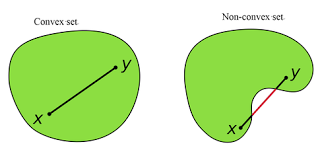
\includegraphics[width=.9\linewidth]{./img/convex_set.png}
\caption{\label{fig:orge8bafe1}
A convex set (gtMath March 2016) \cite{convex_set_img}}
\end{figure}

A convex function on the other hand is simply a function where the entire line
segment between any two points on the graph is above the or on the graph. This
is the part of convex optimisation that determines the fact that the local
minimum is a global minimum. Convex functions are extremely common in the field
of mathematics such as the quadratic function \(x^2\) and the exponential function
\(e^x\). 

Convex optimisation is therefore a relatively simple concept to understand and
is clearly seen to be a very useful and efficient method of accurately and
quickly finding solutions to minimisation problems.
\section{Hyperplane Projection}
\label{sec:org33e0483}
\subsection{Variational Inequality Problem}
\label{sec:orgcb50b98}
The hyperplane projection method is a tool for solving problems that suit the
criteria of a variational inequality problem so first that must be explained
before moving onto the concept of the solution to such a problem.

A variational inequality is an inequality that involves a functional that must
be solved for all variables in a set, usually a convex set. As a side note,
although this problem also involves a convex set like the convex optimisation
problem, the functional is not a convex function and therefore convex
optimisation does not apply in this instance. A functional is a a function that
maps a vector space onto its underlying field of scalars. Often this vector
space can be a series of functions, meaning that the functional takes a function
as an argument and can be interpreted as a function of functions. This is
similar to the Haskell idea of higher order functions, where a single higher
order function can be used to operate on multiple functions and perhaps capture
some other important piece of data for a given system.

The origin of, and primary application of, variational inequality problems is in
the field of finding solutions of equilibrium in a given system. As we'll see
later on in the implementation section of this report, finding the state of Nash
Equilibrium between the different suppliers that take part in the game requires a
state of equilibrium. Therefore it can be easily inferred that the variational
inequality problem is applicable and the problem can be solved as such using a
method appropriate for such a problem.

The hyperplane projection method defined here also stipulates that the
underlying functional involved in the problem must meet a certain monotonicity
criteria. Monotonicity is a property of a function that says that the function
must either be non-decreasing or non-increasing. The function does not have to
be constantly increasing or decreasing but for example if it is increasing then
it cannot decrease or vice versa in order to be deemed monotonic. This can be
represented mathematically as \(f(x) <= f(y) \forall x <= y\) or \(f(x) >= f(y) \forall z <=
y\). Functions that cleave to this mould are called monotonically increasing and
monotonically decreasing respectively. 
\subsection{Hyperplane Projection Method}
\label{sec:org7596192}
Having covered a number of the prerequisites for using a hyperplane projection
method, the method itself can be explained. The version I looked at was
developed by Solodov and Svaiter and is called the Solodov and Svaiter
Hyperplane Projection Method (SSHPM) \cite{solodov1999new}. Figure 6.2 will be
referred to as a part of the explanation.

\begin{figure}[htbp]
\centering
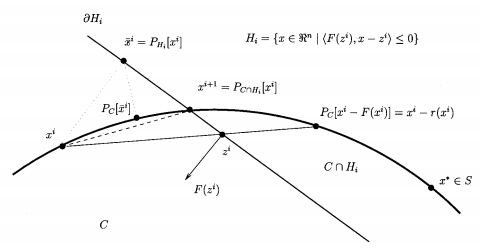
\includegraphics[width=.9\linewidth]{./img/SSHPM.png}
\caption{\label{fig:org5ec6eaf}
Solodov and Svaiter Hyperplane Projection Method}
\end{figure}

The curve in the figure describes the functional in the variational inequality
(VE) problem. This method uses the projection operator \(P_C[x] := arg min ||y -
x||\) where \(y \in C\). Suppose we have a point \(x^i\) which is the current approximation of
the solution to the VE problem involving the set \(C\) and the functional \(F\).
First we calculate a a projection point \(P_C[x^i - F(x^i)]\). The segment between
\(x^i\) and \(P_C[x^i - F(x^i)]\) is searched for a point \(z^i\), using a linesearch
method like the Armijo linesearch method \cite{armijo1966minimization}, such that
a hyperplane \(\delta H_i\) (using the definition of \(H_i\) as defined in figure 6.2)
strictly separates \(x^i\) from any solution \(x^*\) of the problem. The next
approximation to the solution \(x^{i+1}\) is calculated by projecting \(x^i\) onto the
intersection of the set \(C\) and the halfspace \(H^i\) that contains the solution
set using \(P_{C \cap H_i}\).

The benefit of this solution is that each iteration of the method only requires
two projections which makes it computationally efficient, the first to calculate
the hyperplane \(H_i\) and another onto the intersection \(C \cap H^i\) to find the next
iterate in finding the solution. Later on in the Implementation section, the
application of this method will be discussed in further detail.
\part{Implementation}
\label{sec:org64c2fde}
\chapter{Design}
\label{sec:org7dc2416}
\section{Games vs Auctions}
\label{sec:orgd5b7e57}
In the background section of this report both the concepts of Auctions and Game
Theory as both were considered as potential candidates for the management system
to match supply and demand in a nanogrid system. Ultimately however, a
non-cooperative game was chosen as the prime candidate for the smart grid in
this project. It is important to first consider the reasons as to why this
choice was made before explaining how the game was designed.

In the process of investigation of auctions and game theory, certain
similarities stood out between the two management systems. Ultimately all actors
within either of these systems are trying to maximise their utility, a scalar
value that is determined based on a number of key variables that each actor
considers pertinent to their operation. In the case of a model such as this one,
where a price value is involved, the utility of any given actor is usually
modelled as a balance between any profit that the unit could make versus some
kind of risk factor of selling too much at any one given time. In this regard,
the modelling of any actors within the grid would end up being the same on a
conceptual level and only the interactions between them would change based on
what kind of system was chosen.

As has been outlined in previous sections, one of the main criteria for the
nanogrid system, was that of minimal sharing of information between actors in
the grid. This was to decrease the size of packets exchanged between nodes in
the network as well as to hopefully decrease the number of packets sent between
each other in order to improve the efficiency of such a system such that it
might be practical for a real world scenario. Therefore the focus was on a
system that would fit this design. Every auction that was investigated as part
of this report had a crucial element of either all nodes being aware of the each
others' private information or at the very least the central node needed to have
all this information to hand. Therefore a non-cooperative game seemed more
appropriate based off this particular design. 
\section{System Design}
\label{sec:orgf1c09f6}
In this section I will discuss a brief overview of the operation of the system
implemented in this project. Below in Figure 7.2 is a basic flowchart of a
single iteration of the operation of the system, followed by a brief summary of
each step. The summary below assumes that all the nodes within the network have
connected with one another already, although in my code submission there is an
extra step to ensure that the system process doesn't start until the user
decides that it should so that the system can be monitored on a step by step
basis. Figure 7.1 is a simple diagram of the connections between different
actors within the system.

\begin{figure}[htbp]
\centering
\includegraphics[width=.9\linewidth]{./img/basic_network.png}
\caption{\label{fig:org01daa17}
Simple diagram to understand the connections between the different actors involved in the system in a given iteration}
\end{figure}

\begin{figure}[htbp]
\centering
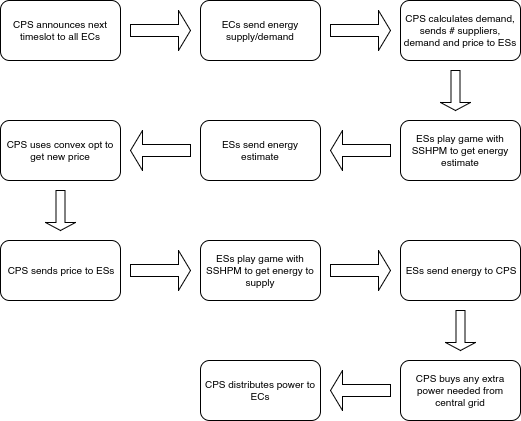
\includegraphics[width=.9\linewidth]{./img/design.png}
\caption{\label{fig:orgc280f7a}
Flow chart depicting the operation of the system in terms of the Central Power Station (CPS), Energy Consumers (ECs) and Energy Suppliers (ESs) in a single iteration}
\end{figure}

An iteration of the system is conducted to match supply and demand for in a
nanogrid situation for a given upcoming timeslot. Some kind of system where a
consumer can predict their energy usage for the next timeslot is presumed to be
in place. The suppliers of course know what their own supply of energy is as
well as having a caution variable \(c \in (0, 1)\). The caution value determines how
willing they are to sell larger amounts of energy, a low caution value
representing a willingness to sell more energy and a high value standing for a
more conservative supplier.

The operation begins with the Central Power Station (CPS) announcing a timeslot
to all consumers and all suppliers within the network. At the beginning the CPS
doesn't know who is a consumer and who is a supplier in order to accommodate the
situation where a consumer has proactively bought too much energy in
anticipation of needing it or has been instructed by some logic to sell excess
energy into the grid. Each Energy Consumer (EC) then notifies the CPS as to
whether it is in need of energy or whether it has energy to sell and if it's the
case of the former then it also sends how much energy it requires. Figure 7.1
shows the situation where ECs within the grid have already made it clear as to
whether they are a supplier or a consumer for this particular timeslot.

The CPS then simply sums the total demand and can begin the game. It sends to
the total demand, the total amount of money it has available to give and the
number of suppliers within the system to each Energy Supplier (ES). The total
price is calculated naively by multiplying the current price per unit that is
offered by the central grid by the number of units of energy required by the
consumers within the nanogrid. A standard unit would be kWh. Each ES first
calculates how much energy it can be offered by dividing the total price by the
number of players. Each one then uses the SSHPM optimisation method to determine
an estimate for the energy it is willing to give to the CPS at that price and
sends that estimate to the CPS. The functional used as part of the SSHPM is the
utility function of each EC and the set of values being mapped over is a one
dimensional vector space that goes from zero to whatever the total energy of
each EC is.

The CPS then receives each ES's energy estimate. From this it is able to
estimate how willing each ES is to giving more or less energy. It cannot work
out the private store or the caution of each ES but rather understands the ratio
that exists between all the different players involved. The CPS then uses its
own utility function and the vector of energy estimates from each ES as the
inputs to a convex optimisation problem. A disciplined convex optimisation
method is employed \cite{grant2006disciplined} as any standard convex optimisation 
technique is all that is required and the Python solver CVXPY \cite{diamond2016cvxpy} was readily
available. A new vector of prices per ES is generated and each one is sent to
each ES. This is the actual price that each ES receives.

The ESs then play another game using their utility functions and the new price
that they have been offered by the CPS and try to find the actual amount of
energy that they are willing to give away using SSHPM. This energy is then sent
to the CPS. The CPS then sums the total of energy that has been provided at that
time. If this energy matches the total demand of the consumers in the nanogrid,
then the energy is simply supplied to those who need it, on a first come first
serve basis. However, if the supply does not reach the demand then the CPS buys
the extra power that is needed from the central power grid as seen in Figure
7.1. This system accepts the fact that it may not be able to supply all
consumers within the nanogrid using solely local sources that exist within its
own grid. Once the supply matches the demand, the power is then distributed as
before. The process then starts again ahead of the next timeslot to ensure that
everyone that needs power during that time is supplied.
\section{Game Design}
\label{sec:orge6b6536}
First some of the key components of the game as well as a brief overview of how
it  is conducted will be explained and then after that, the game will be
discussed ins and outs will be discussed in further detail The game played
between all of the ESs that are trying to receive remuneration for the energy
they are willing to offer is played across two steps. First of all the ESs use
their utility functions along with a number of other important variables such as
their energy capacity \(E_n\), caution \$c\(_{\text{n}}\) and the current price offer \(p_n\) in
order to determine their new estimate for how much energy they are willing to
offer to the CPS \(e_n\), where \(n \in N\), N being the set of all ESs taking part in
the nanogrid. Next they use that energy estimate to calculate a slack variable
\(\varepsilon_n\) which is a variable indicating the amount of energy it is willing to offer
without giving up any private information. These slack variables are derived
from the ES's utility functions which will be discussed in the next section. The
slack variables are used by the CPS to determine Nash Equilibrium within the
game, namely this is when all of the slack variables are equal. Once this state
of equilibrium is reached, then the CPS asks for the energy offer from each of the
ESs.

When the hyperplane projection is initially calculated there is a small piece of
logic that determines what slack variable is sent to the CPS as well as what
energy should be offered. If the projection is equal to zero then \(\varepsilon_n = E_n -
2c_{n}e_{n} + p_n\). Otherwise the second part of the hyperplane projection method is
run, where the halfspace is determined and from that a new projection is worked
out. In this case the slack variable sent back to the CPS is \(\varepsilon_n = E_n - e_n +
p_n\). These slack variables are then sent to the CPS. If the slack variables are
all equal, as previously mentioned, then the game has reached the state of Nash
Equilibrium and the ESs are informed to end their iterations and they instead
send back the amount of energy they are offering. If the slack variables are not
equal then the CPS instructs the ESs to perform another iteration of the SSHPM.
\section{Utility Functions}
\label{sec:org1a38a77}
\subsection{EC Utility Function}
\label{sec:org16a048f}
Each EC has a utility function that is used as the functional in the the
hyperplane projection optimisation. The utility function in question takes into
account the energy that EC \(n\) has stored \(E_n\), the price being offered to it
\(p_n\), the caution value of that EC \(c_n\) and the energy that it is offering \(e_n\).
$$ U(e_n, E_n, p_n) = p_{n}e_{n} + (E_{n} - c_{n}e_{n})e_{n} $$ 
This utility function is based on the profit that the EC could get when it is
supplying energy, that is \(p_{n}e_{n}\). \((E_{n} - c_{n}e_{n})e_{n}\) represents the loss that the
EC incurs by giving away a certain amount of power. Ultimately the system is
trying to maximise the utilities of all ECs in the nanogrid, where the sum of
all offered energies is less than or equal to the energy deficiency (demand) of the
system for a given timeslot \(E_{def}\), that is $$\sum_n e_n <= E_{def}$$.
\subsection{CPS Utility Function}
\label{sec:org4a4f6ee}
The CPS has its own utility function that serves as the convex function for the
convex optimisation problem in trying to find appropriate prices for each of the
ESs that have submitted energy estimates for how much they are willing to offer.
The function is represented as a minimisation problem in terms of the energy
that each ES is offering \(e_n\), the price that the CPS would offer for that
energy \(p_n\) and two scalar values \(a_n\) and \(b_n\)  that account for the costs
associated with storing and transmitting the energy.

$$min_p L(p,e) = min_{p_{n}} \sum_n(e_{n}p_n^r + a_{n}p_{n} + b_n), subject to \sum_n p_n = P, p_{min}
<= p_n <= p_{max}$$

For each ES, the CPS is trying to find the value of \(p_n\) that will give the
smallest value. However all values of \(p_n\) must sum to be equal to the value of
\(P\), the total price that the CPS is willing to pay. As can be seen in this
model, the system doesn't pay any less for power overall, but rather
incentivises all suppliers of electricity to try to match the demand in
question. Another caveat of the minimisation problem is that \(p_n\) must be
between the values of \(p_{min}\) and \(p_{max}\). This simply means that there is a
minimum and a maximum value that the CPS is willing to pay for energy.
\chapter{Application}
\label{sec:org245e458}
\section{Python Twisted Framework}
\label{sec:org3394740}
In the course of this project the Python Twisted Framework \cite{twistedpython}
was used in order to implement a network between the CPS and the ECs. The
Twisted Framework has a number of layers in order to abstract out the problem
for the user so that they only need care about their own application
\cite{kinder2005event}. It also has a number of inbuilt functions so that the
programmer does not have to care about things like sockets that are very tricky
and are far removed from the problem trying to be solved in this project.

Both the Client and the Server have two main layers where all the Twisted magic
happens, the Factory layer and the Protocol layer. Essentially the Factory layer
contains all of the persistent information of any given network actor and the
Protocol layer contains actions and information for every connection made by
that actor. In the code produced as part of this project, the factories of the
CPS and the ECs were mostly used to store the values of variables pertinent to
each of them such as the price vectors for the CPS and the energy storage for
each of the ECs.

The majority of the logic that controls both the CPS and ECs was contained
within separate Finite State Machine (FSM) files which were connected to their
respective Protocol files the FSM only changes state based on the inputs it
receives from any given connection. It was easiest to abstract the problem out
in this fashion for ease of reading and understanding of the code for both the
programmer and any potential readers. Each EC and the CPS is finally wrapped by
a simple run script that just sets up the factory from which everything else is
run. In each section below, the FSM of both the ECs and the CPS will be examined
as the system is conducted in the same fashion for both, where the protocol
calls a different function in the FSM depending on the state of the actor at
that time.
\section{Client (EC)}
\label{sec:org72aca76}
\subsection{Idle State}
\label{sec:org83fb78e}
The idle state is merely a state for in between operations of the system, where
no game is being played. In this project it was also used as an initial state
before the user decides to start the game. When a new game is started by the
CPS, it notifies each EC to move into the start state.
\subsection{Start State}
\label{sec:org4f2b9df}
The start state is where the EC sends a message to the CPS to inform it as to
whether it is a supplier or a consumer for the upcoming timeslot. If it is a
consumer then it also sends the amount of energy that it requires at that time.
Also if an EC in the nanogrid requires no energy for the next timeslot, then it
simply puts itself back into the idle state, awaiting the next timeslot when it
might need or be able to supply energy. An EC moves to the Estimate 1 State if
it is a supplier and to the receive state if it is a consumer.
\subsection{Estimate 1 State}
\label{sec:orge0ff1d3}
This state is used for when the ESs are playing the game and making their first
estimate of how much energy they are willing to offer to the CPS. In this state,
if an ES is told to "End" its iterations then it moves to the second estimation
state (Estimate 2 State). Otherwise it uses the hyperplane projection method
solver (SSHPM Implementation) that was developed as part of this project and
sends a slack variable to the CPS, used in determining Nash Equilibrium for the
game. 
\subsection{Estimate 2 State}
\label{sec:org8937eeb}
The Estimate 2 State is more or less the exact same as Estimate 1 State except
that when it receives the "End" message, it instead moves back to the idle
state, having successfully supplied energy to the CPS and having been
remunerated for that energy. If it doesn't receive the end message then it uses
SSHPM to calculate a new slack variable and continues playing the game.
\subsection{Receive State}
\label{sec:org2e8146c}
The Receive State is the state for any consumers for the current timeslot. An EC
stays in this state until the operation of the system has been completed and the
energy is distributed to it accordingly. Once it receives this energy, it
returns to the Idle state in order to wait for the next timeslot.
\subsection{SSHPM Implementation}
\label{sec:orgb9dddef}
The SSHPM implementation caused the greatest amount of difficulty as part of
this final year project. The paper \cite{solodov1999new} details a complex and
dense mathematical algorithm that was difficult to grasp and to implement. The
functions with the SSHPM.py file follow the steps in the algorithm defined by
Solodov and Svaiter.
\section{Server (CPS)}
\label{sec:org52bfa49}
\part{Conclusion}
\label{sec:org947c8c8}
\chapter{Results}
\label{sec:orge8d388d}
\chapter{Assessment}
\label{sec:orga4579ba}
\chapter{Future Work and Continuations}
\label{sec:org8bfe396}

\printbibliography
\appendix
\end{document}